\begin{frame}{Akash feedback on 20.09.2018}
\begin{itemize}
\item Algorithm to automatically identifying combinational XOR-chains at primary outputs, and encrypting them
\item Algorithm to encrypt the scan-chain
\item Quantify runtime and functional output corruption
\item Implementation on ISCAS'85 and OpenSPARC circuits
\item \alert{Idea}: Since there are primary output XOR-chains for ALUs (used for PC, Branch target calculator, Execution units etc.), this idea will lock the processor successfully
\item Algorithm for selective flip-flop locking, to minimize area overhead due to sequential locking
%\item Target DAC (if more algorithmic work involved) or HOST
\end{itemize}
\end{frame}

\begin{frame}{Next steps}
\begin{itemize}
%\item For selectively locking flip-flops, are some flip-flops more special than others to lock (in terms of shooting-up SAT-running-time and thus making decryption harder) ?
\item Algorithm to decode correct combinational key, given sequential key
\end{itemize}
\end{frame}

\begin{frame}{Algorithm to decrypt correct combinational key}
\begin{itemize}
\item Step 1: Run SAT solver on scan-unrolled combinational circuit, to find sequential key
\item Step 2: Isolate combinational circuit, apply combinational portion of key, and add virtual key gates at POs, and run SAT solver
\item Step 3: Apply virtual key values, and make combinbational key unknown again, and run SAT-solver
\end{itemize}
\end{frame}

\begin{frame}{\texttt{c17} circuit}
       \begin{figure}
                \begin{center}
                \label{fig:c17-c}
                \caption{\texttt{c17} combinational circuit}
                        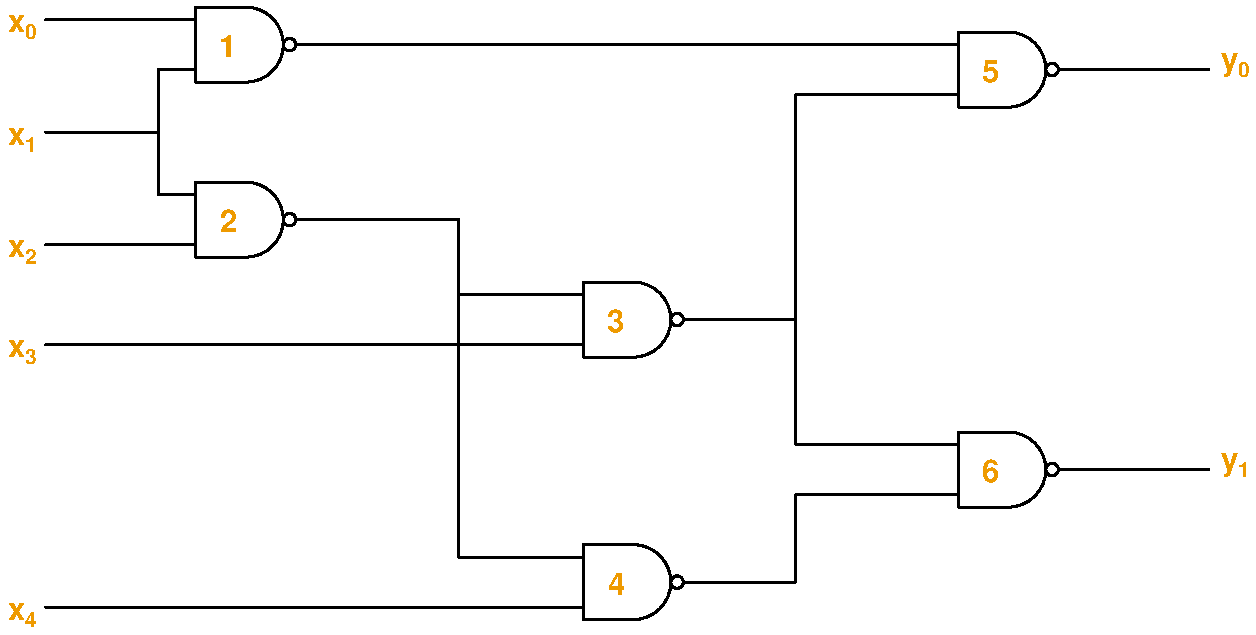
\includegraphics[scale=0.3]{fig/c17_original.pdf}
                \end{center}
        \end{figure}
\end{frame}

\begin{frame}{\texttt{c17} circuit with sequential locking}
       \begin{figure}
                \begin{center}
                \label{fig:c17-s-l}
                \caption{\texttt{c17} circuit with sequential locking}
                        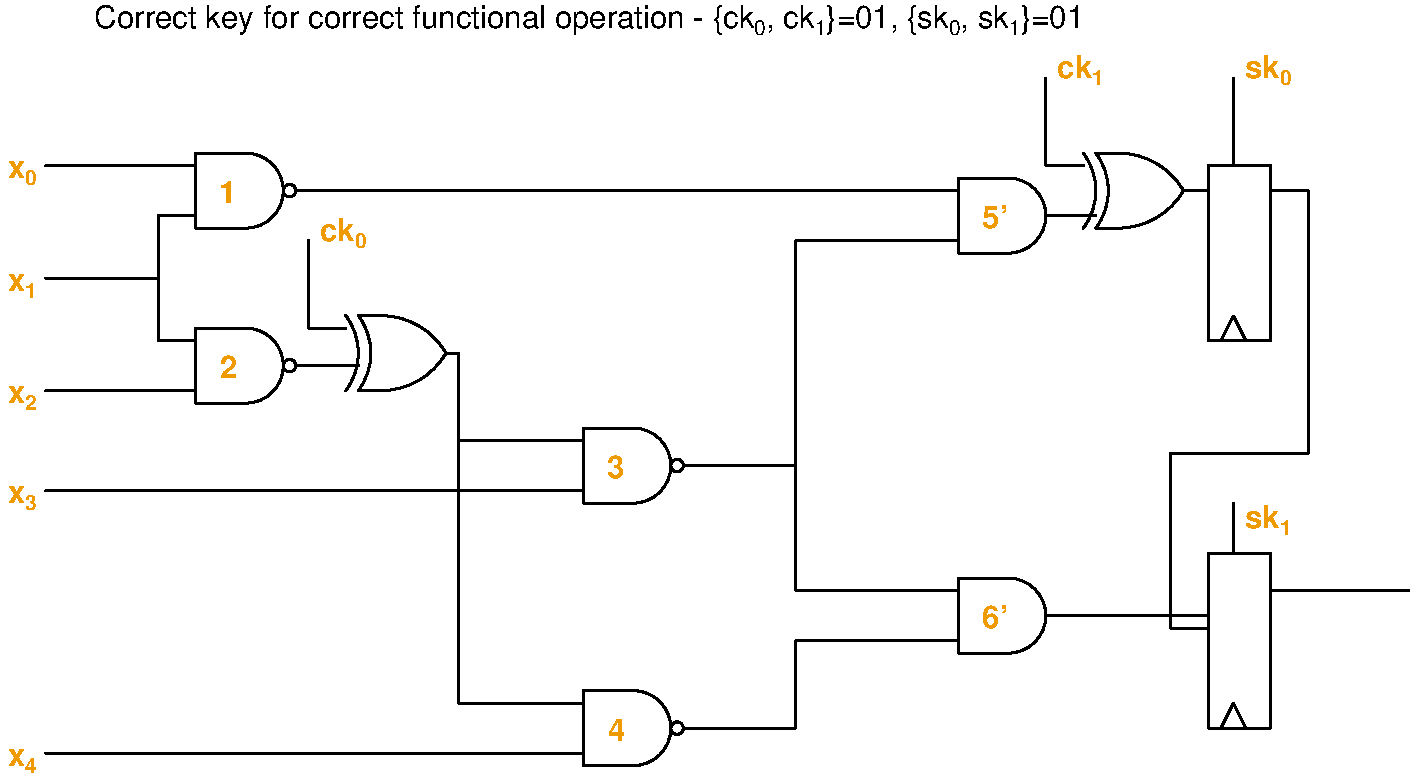
\includegraphics[scale=0.3]{fig/c17_sequentially_locked.pdf}
                \end{center}
        \end{figure}
\end{frame}


\begin{frame}{\texttt{c17} circuit with scan unroll and Step 1}
       \begin{figure}
                \begin{center}
                \label{fig:c17-s-l-Algo-Step1}
                \caption{\texttt{c17} circuit with scan unroll and Step 1}
                        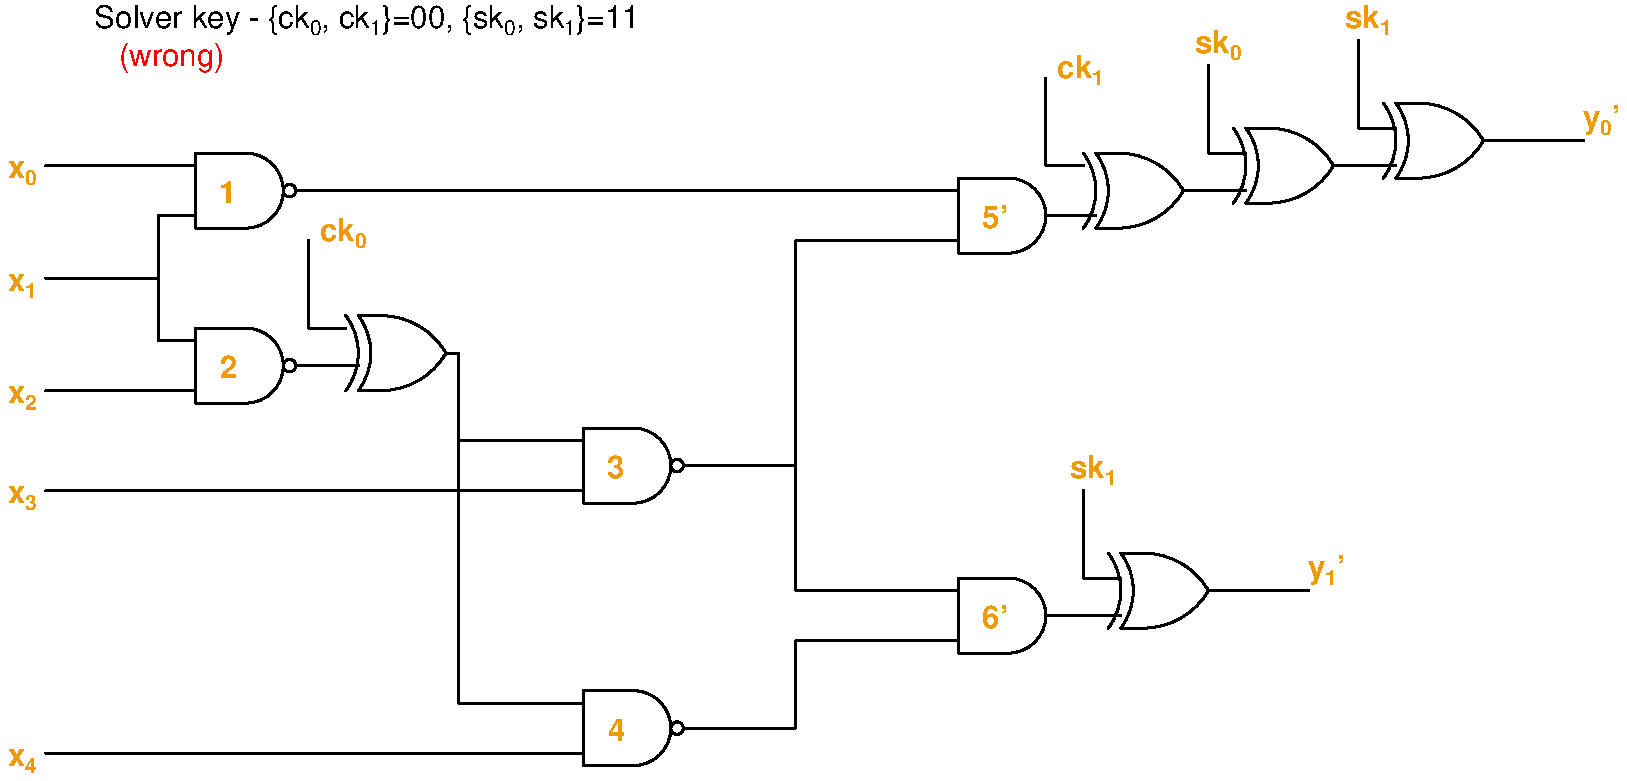
\includegraphics[scale=0.3]{fig/c17_sequentially_locked_scan_unrolled_Algo_Step1.pdf}
                \end{center}
        \end{figure}
\end{frame}

\begin{frame}{\texttt{c17} circuit with scan unroll and Step 2}
       \begin{figure}
                \begin{center}
                \label{fig:c17-s-l-Algo-Step2}
                \caption{\texttt{c17} circuit with scan unroll and Step 2}
                        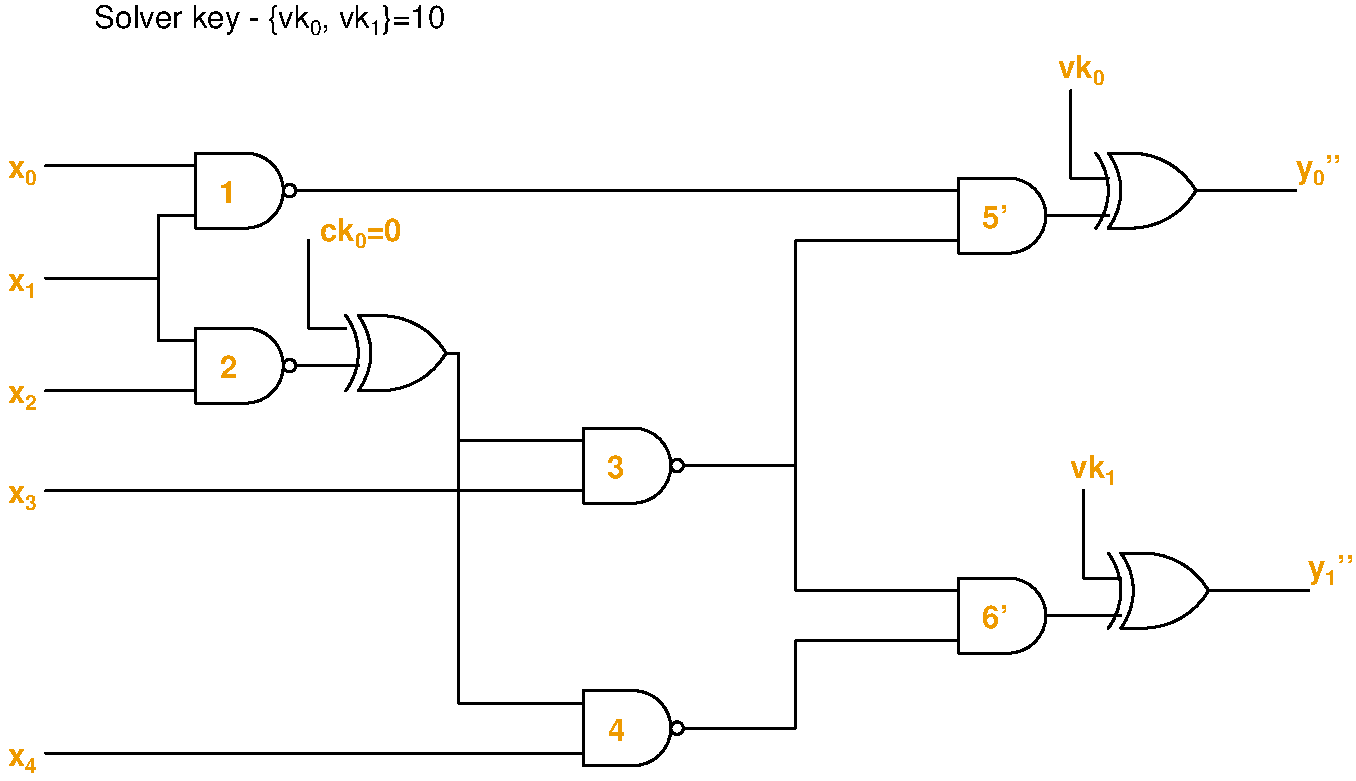
\includegraphics[scale=0.3]{fig/c17_sequentially_locked_scan_unrolled_Algo_Step2.pdf}
                \end{center}
        \end{figure}
\end{frame}

\begin{frame}{\texttt{c17} circuit with scan unroll and Step 3}
       \begin{figure}
                \begin{center}
                \label{fig:c17-s-l-Algo-Step2}
                \caption{\texttt{c17} circuit with scan unroll and Step 3}
                        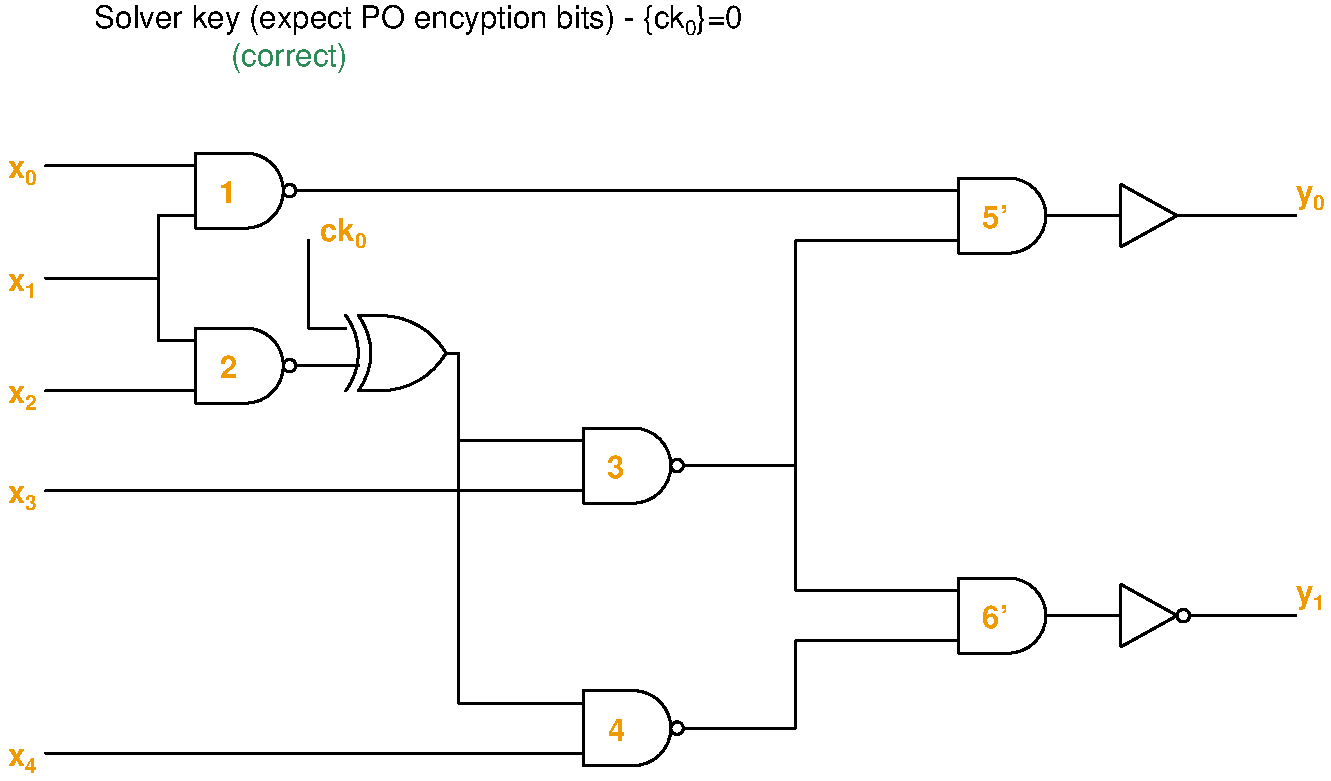
\includegraphics[scale=0.3]{fig/c17_sequentially_locked_scan_unrolled_Algo_Step3.pdf}
                \end{center}
        \end{figure}
\end{frame}

\begin{frame}{Observation}
\begin{itemize}
\item In principle, the Algorithm can solve for the correct combinational key
\item However, we do not have the reference correct combinational circuit for Step 2, since we only have access to scan data on the activated IC
\item Hence Algorithm is not feasible
\item Thus, we need to make $2^M$ (for circuit with M flip-Flops) observations. 
\item For \texttt{c880} circuit, $M=26$, thus running time = $2^{26}*0.04s = 3, 355, 433 s  \approx 1 month $
\item \texttt{c880} has 105 primary inputs (PIs); if we add flip-flops at PIs as well, running time increases $2^{105}\times$ further. 
\end{itemize}
\end{frame}


\begin{frame}{Experimental evaluation}
\begin{itemize}
\item Formulate the sequential locking problem, as an instance of the logic locking problem, and solve for the sequential key
\item Extract the combinational portion of the key, and apply to the combinational portion of the circuit, and check if it is formally equivalent to original circuit
\item If \alert{YES}, it means decrypted decrypted key produces \alert{correct} functional outputs when applied to the encrypted circuit
\item If \alert{NO}, it means decrypted decrypted key produces \alert{corrupt} functional outputs when applied to the encrypted circuit
\end{itemize}
\end{frame}

\begin{frame}{Results for $5\%$ combinational (random) encryption and encrypting all output flip-flops}
\begin{itemize}
\item Decrypted key produces correct functional outputs : \texttt{apex2}, \texttt{apex4}, \texttt{c432}, \texttt{c499} 
\item Decrypted key produces corrupt functional outputs : \texttt{c880}, \texttt{c7552}, \texttt{c1908}, \texttt{c1355}, \texttt{c5315}, \texttt{c2670}, \texttt{c3540}, \texttt{dalu}, \texttt{des}, \texttt{ex1010}, \texttt{ex5}, \texttt{i4}, \texttt{i7}, \texttt{i8}, \texttt{i9}, \texttt{k2}, \texttt{seq}
\item Success rate : $\frac{17}{21}$ cases \alert{$\approx 81\%$}
%\item \alert{ 100\%} correlation between presence of XOR-type encryption at POs and success in functional output corruption
\end{itemize}

\end{frame}

\begin{frame}{Results for $5\%$ target combinational (random and PO) encryption and encrypting all output flip-flops}
\begin{itemize}
\item Decrypted key produces correct functional outputs : \alert{Nil}
\item Decrypted key produces corrupt functional outputs : \texttt{c880}, \texttt{c7552}, \texttt{c1908}, \texttt{c1355}, \texttt{c5315}, \texttt{c2670}, \texttt{c3540}, \texttt{dalu}, \texttt{des}, \texttt{ex1010}, \texttt{ex5}, \texttt{i4}, \texttt{i7}, \texttt{i8}, \texttt{i9}, \texttt{k2}, \texttt{seq}, \texttt{c432}, \texttt{c499}, \texttt{apex2}, \texttt{apex4}
\item Success rate : $\frac{21}{21}$ cases \alert{$= 100 \%$}
\end{itemize}

\end{frame}

\begin{frame}{Results for $5\%$ combinational (DAC'12 fault analysis based) encryption and encrypting all output flip-flops}
\begin{itemize}
\item Decrypted key produces correct functional outputs : \texttt{i4}, \texttt{i7}, \texttt{i8}, \texttt{i9}, \texttt{apex2}, \texttt{apex4}, \texttt{seq}, \texttt{k2}, \texttt{dalu}, \texttt{ex1010}, \texttt{ex5}, \texttt{des}, \texttt{c432}, \texttt{c499}, \texttt{c7552}, \texttt{c1908}, \texttt{c1355}, \texttt{c3540}
\item Decrypted key produces corrupt functional outputs : \texttt{c880}, \texttt{c5315}
\item \texttt{c2670} run in progress ($> 48$ hours). The SAT-attack paper mentions they could not decrypt this benchmark. 
\item Success rate : $\frac{2}{20}$ cases \alert{$= 10\%$}
%\item \alert{ 100\%} correlation between presence of XOR-type encryption at POs and success in functional output corruption
\end{itemize}
\end{frame}

\begin{frame}{Results for $5\%$ combinational (DAC'12 Fault analysis + PO) encryption and encrypting all output flip-flops}
\begin{itemize}
\item Decrypted key produces correct functional outputs :    \texttt{apex2} (only 3 POs),   
\item Decrypted key produces corrupt functional outputs : \texttt{i4}, \texttt{i7}, \texttt{i8}, \texttt{i9}, \texttt{apex4}, \texttt{k2},  \texttt{seq}, \texttt{dalu}, \texttt{des},  \texttt{ex1010}, \texttt{ex5}, \texttt{c432}, \texttt{c499}, \texttt{c880}, \texttt{c1355}, \texttt{c3540}, \texttt{c5315}, \texttt{c1908},  \texttt{c7552} 
\item Success rate : $\frac{19}{20}$ cases \alert{$= 95\%$}
%\item \alert{ 100\%} correlation between presence of XOR-type encryption at POs and success in functional output corruption
%\item \textttt{c7552} took 1 hr runtime
\end{itemize}
\end{frame}

\begin{frame}{Results for $5\%$ combinational (IOLTS'14) encryption and encrypting all output flip-flops}
\begin{itemize}
\item Decrypted key produces correct functional outputs : \texttt{apex2}, \texttt{apex4}, \texttt{i4}, \texttt{i7}, \texttt{i8}, \texttt{i9}, \texttt{ex1010}, \texttt{ex5}, \texttt{k2}, \texttt{seq}, \texttt{dalu}, \texttt{des}, \texttt{c432}, \texttt{c499}, \texttt{c1908}, \texttt{c1355}, \texttt{c5315}, \texttt{c7552}, \texttt{c3540}, \texttt{c880}, \texttt{c2670}
\item Decrypted key produces corrupt functional outputs : \alert{Nil}
\item Success rate = $\frac{0}{21}$ cases = \alert{0\%}
%\item In other words 100\% success in decrypting the correct combinational key
%\item Exact (bit-by-bit) combinational key is getting recovered: looks like equivalence classes don't exist in AND-type or OR-type encryption (IOLTS'14)
\end{itemize}
\end{frame}

\begin{frame}{Results for $5\%$ combinational (IOLTS'14 and PO) encryption and encrypting all output flip-flops}
\begin{itemize}
\item Decrypted key produces correct functional outputs :  \alert{Nil}  
\item Decrypted key produces corrupt functional outputs :  \texttt{c2670}, \texttt{c3540}, \texttt{c5315}, \texttt{c7552}, \texttt{k2}, \texttt{seq}, \texttt{ex5}, \texttt{ex1010},  \texttt{apex2}, \texttt{apex4}, \texttt{c432}, \texttt{c499}, \texttt{c880}, \texttt{i4},  \texttt{i7}, \texttt{i8},  \texttt{i9},  \texttt{c1908}, \texttt{c1355}, \texttt{dalu}, \texttt{des}
\item Success rate = $\frac{21}{21}$ cases = \alert{100\%}
%\item In other words 100\% success in decrypting the correct combinational key
%\item Exact (bit-by-bit) combinational key is getting recovered: looks like equivalence classes don't exist in AND-type or OR-type encryption (IOLTS'14)
\end{itemize}
\end{frame}

\begin{frame}{Results for $5\%$ combinational (TOC13'XOR) encryption and encrypting all output flip-flops}
\begin{itemize}
\item Decrypted key produces correct functional outputs :  \texttt{i9}, \texttt{des}, \texttt{c432}, \texttt{c499}, \texttt{c3540}, \texttt{c880}, \texttt{c1908}
\item Decrypted key produces corrupt functional outputs : \texttt{apex2}, \texttt{apex4}, \texttt{i4}, \texttt{i7}, \texttt{i8}, \texttt{ex1010}, \texttt{ex5}, \texttt{k2}, \texttt{seq}, \texttt{dalu}, \texttt{c1355}, \texttt{c5315}, \texttt{c2670}, \texttt{c7552} 
\item Success rate = $\frac{14}{21}$ cases \alert{$\approx 67\%$}
%\item \alert{ 100\%} correlation between presence of XOR-type encryption at POs and success in functional output corruption
%\item For \texttt{c1355}, no XOR-type key-gate right at PO. 
%\item For \texttt{c7552}, 11 hrs runtime
\end{itemize}
\end{frame}


\begin{frame}{Results for $5\%$ combinational (TOC13'XOR and PO) encryption and encrypting all output flip-flops}
\begin{itemize}
\item Decrypted key produces correct functional outputs :  \alert{Nil}  
\item Decrypted key produces corrupt functional outputs : \texttt{apex2}, \texttt{apex4}, \texttt{i4}, \texttt{i7}, \texttt{i8}, \texttt{ex1010}, \texttt{ex5}, \texttt{k2}, \texttt{seq}, \texttt{dalu}, \texttt{c1355}, \texttt{c5315}, \texttt{c2670}, \texttt{c7552}, \texttt{i9}, \texttt{c432}, \texttt{c499}, \texttt{c1908}, \texttt{c880}, \texttt{c3540}, \texttt{des},
\item Success rate = $\frac{21}{21}$ cases \alert{$= 100\%$}
\end{itemize}
\end{frame}


\begin{frame}{Results for $5\%$ combinational (TOC13'MUX) encryption and encrypting all output flip-flops}
\begin{itemize}
\item Decrypted key produces correct functional outputs : \texttt{apex2}, \texttt{i4}, \texttt{i7}, \texttt{i8}, \texttt{i9}, \texttt{ex1010}, \texttt{ex5}, \texttt{k2}, \texttt{seq}, \texttt{dalu}, \texttt{des}, \texttt{c432}, \texttt{c499}, \texttt{c1355}, \texttt{c5315}, \texttt{c7552}, \texttt{c3540}, \texttt{c2670}, \texttt{c880}, \texttt{c1908}
\item Decrypted key produces corrupt functional outputs : \texttt{apex4}
\item Success rate = $\frac{1}{21}$ cases \alert{$\approx 5\%$}
\end{itemize}
\end{frame}

\begin{frame}{Results for $5\%$ combinational (TOC13'MUX and PO) encryption and encrypting all output flip-flops}
\begin{itemize}
\item Decrypted key produces correct functional outputs : \alert{Nil}
\item Decrypted key produces corrupt functional outputs : \texttt{apex4}, \texttt{apex2}, \texttt{i4}, \texttt{i7}, \texttt{i8}, \texttt{i9}, \texttt{ex1010}, \texttt{ex5},  \texttt{k2}, \texttt{seq},  \texttt{dalu},  \texttt{des} ($\approx$ 2 hours), \texttt{c432}, \texttt{c499}, \texttt{c1355}, \texttt{c5315}, \texttt{c880}, \texttt{c1908}, \texttt{c3540}, \texttt{c7552}, \texttt{c2670}, 
\item Success rate = $\frac{21}{21}$ cases \alert{$\approx 100 \%$}
\end{itemize}
\end{frame}

%\begin{frame}{Complexity to decrypt correct combinational key}
%\begin{itemize}
%\item If circuit $C$ has $M$ POs, search-space to explore which outputs undergo inversions along scan-chain and which not, is \alert{$2^M$}.
%\item Because of this exponential search-space and typical circuits can have hundreds of POs, it is not possible for SAT-attacker to decrypt correct combinational key, given the decrypted sequential key.
%\end{itemize}
%\end{frame}

\begin{frame}{Theorem}
Using virtual gates (shown in slide 62), it is possible to find portion of correct combinational key (except the encryption bits at POs)
\end{frame}

\begin{frame}{Theorem}
It is not possible to find the encryption bits at POs
\end{frame}

\begin{frame}{Conclusion}
Hence, our methodology in adding XOR-based encryption gates at POs, is ROBUST (in the sense that it is not possible to reformulate and solve for the PO encryption key bits, hence not possible to decrypt the complete combinational key). 
\end{frame}

\begin{frame}{Boundary Encryption- Experiment 1}
\begin{itemize}
\item I have added XOR-type encryption key gates to all 7 outputs of \texttt{c432} circuit and encrypted all output flip-flops
\item The {\em functionally correct key} is \alert{0000000} (singleton equivalence class)
\item However, running ScanSAT on scan unrolled version of above boundary encrypted \texttt{c432} circuit, gave \alert{0010000}, hence corrupting functional output
\item Thus, boundary encryption produces SAT-attack Resilient Circuits. 
\item No need to add key gates deep inside combinational logic. 
\end{itemize}
\end{frame}


\begin{frame}{Boundary Encryption- Experiment 2}
\begin{itemize}
\item Everything same as experiment 1, however number of encrypted POs is variable
\item {7, 6, 5, 4, 3, 2}: decrypted \alert{functionally incorrect key}
\item {1} : decrypted {functionally correct key}
\item So, minimum 2 POs need to be encrypted. This is what I have manually done in all the experiments, across the 21 benchmarks, spanning the 5-encryption-schemes. Hence, the success rate reached \alert{100 \%} by just encrypting just 2-3 POs. 
\end{itemize}
\end{frame}

\begin{frame}{Advantages of Boundary Encryption}
\begin{itemize}
\item We need to add few XOR/XNOR-type encryption key gates, just at POs, and no need to add them deep inside combinational logic. 
\item This makes the encryption scheme very area-efficient. The key gates can be added to timing-uncritical POs. 
\item Area, Timing and Power friendly. 
\item This makes this method seamless integrable to industry practice
\item The method scales easily from IP-level to SoC-level. 
\end{itemize}
\end{frame}

\begin{frame}{Advantages of Boundary Encryption/Locking}
\begin{itemize}
\item Logic Locking techniques lock only the combinational logic, hence vulnerable to scan-based SAT-attack, EDT-Bypass mode; 
\item Scan Locking locks only the scan chains, using Encrypt-Flip-Flop. However, ScanSAT models this as an instance of logic locking problem, hence also vulnerable to SAT-attack; 
\item \alert{Boundary Locking} combines both intelligently, to thwart SAT-attack. 
\item Compare area overhead for all circuits reported in Table II of Encrypt Flip-Flop paper. 
\item Report running times
\end{itemize}
\end{frame}
